\documentclass[tikz,border=4pt]{standalone}
\usetikzlibrary{shapes.geometric, arrows, positioning}
\begin{document}
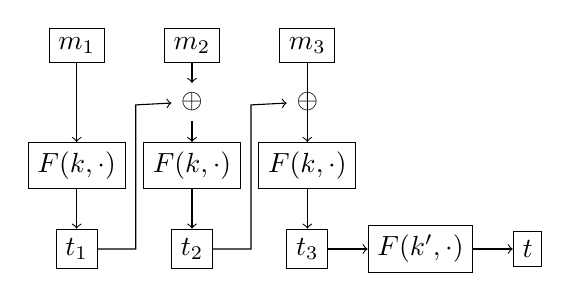
\begin{tikzpicture}
		\node (m0) [draw] {$m_1$};
    \node[below =1cm of m0] (f0) [draw] {$F(k, \cdot)$};
		\node[below =0.5cm of f0] (t0) [draw] {$t_1$};
		\draw [->] (m0) edge (f0) (f0) edge (t0);

		\node[right=0.75cm of m0] (m1) [draw] {$m_2$};
		\node[below =0.25cm of m1] (m1xt0) {$\oplus$};
		\draw [->] (t0) - ++(0.75,0) -- ++(0.75,1.83) -- (m1xt0);
    \node[below =1cm of m1] (f1) [draw] {$F(k, \cdot)$};
		\node[below =0.5cm of f1] (t1) [draw] {$t_2$};
		\draw [->] (m1) edge (m1xt0) (m1xt0) edge (f1) (f1) edge (t1);

		\node[right=0.75cm of m1] (m2) [draw] {$m_3$};
		\node[below =0.25cm of m2] (m2xt1) {$\oplus$};
		\draw [->] (t1) - ++(0.75,0) -- ++(0.75,1.83) -- (m2xt1);
    \node[below =1cm of m2] (f2) [draw] {$F(k, \cdot)$};
		\node[below =0.5cm of f2] (t2) [draw] {$t_3$};
    \node[right=0.5cm of t2] (out) [draw] {$F(k', \cdot)$};
    \node[right=0.5cm of out] (outp) [draw] {$t$};
		\draw [->] (m2) edge (f2) (f2) edge (t2);
    \draw [->] (t2) edge (out);
    \draw [->] (out) edge (outp);
\end{tikzpicture}
\end{document}
